\section{Formulating Recursive Cases}

\begin{Def}[Dynamic Programming]

In recursive algorithms, there are many cases where we repeat 
the same computations multiple times. To reduce this redundancy, we store 
the results of these computations in a table. This is known as \textbf{memoization}. This paradigm of programming is 
called \textbf{dynamic programming}.
\end{Def}
\textbf{Scenario - \textit{Fibonacci Sequence}:} The Fibonacci sequence is defined as $F_n=F_{n-1}+F_{n-2}$, with $F_0=0$ and $F_1=1$. Our 
first 8 terms are $\{0,1,1,2,3,5,8,13\}$. To compute $F_5$, we do $0+1=1$, $1+1=2$, $1+2=3$, and $2+3=5$.\\

\noindent
A recursive approach would be:

\begin{Func}[Slow Fibonacci Sequence - \textit{Fib()}]
    \noindent
    \textbf{Input:} $n$ the index of the Fibonacci sequence we wish to compute.\\
    \textbf{Output:} $F_n$ the $n_{th}$ Fibonacci number.\\

    \vspace{-.5em}
    \begin{algorithm}[H]
        \SetAlgoLined
        \SetKwProg{Fn}{Function}{:}{\KwRet{}}
        \Fn{\textit{Fib}($n$)}{
            \If{$n \leq 1$}{
                \textbf{return} $n$\;
            }
            \Else{
                \textbf{return} $\textit{Fib}(n-1)+\textit{Fib}(n-2)$\;
            }
        }
    \end{algorithm}
    \rule{\textwidth}{0.4pt}
    \textbf{Time Complexity:} $O(2^n)$. Since line 6 depends on both calls, we reflect such in our recurrence relation, $T(n)=T(n-1)+T(n-2)+O(1)$, Theorem (\ref{theo:master}). Since we make 
    calls of size $n-1$ and $n-2$, both $O(n)$ we have an exponential time complexity $O(2^n)$. 
\end{Func}

\newpage
\noindent
When we unravel the recursion tree, we see plenty of redundancies:

\begin{figure}[h]


\hspace{5em} 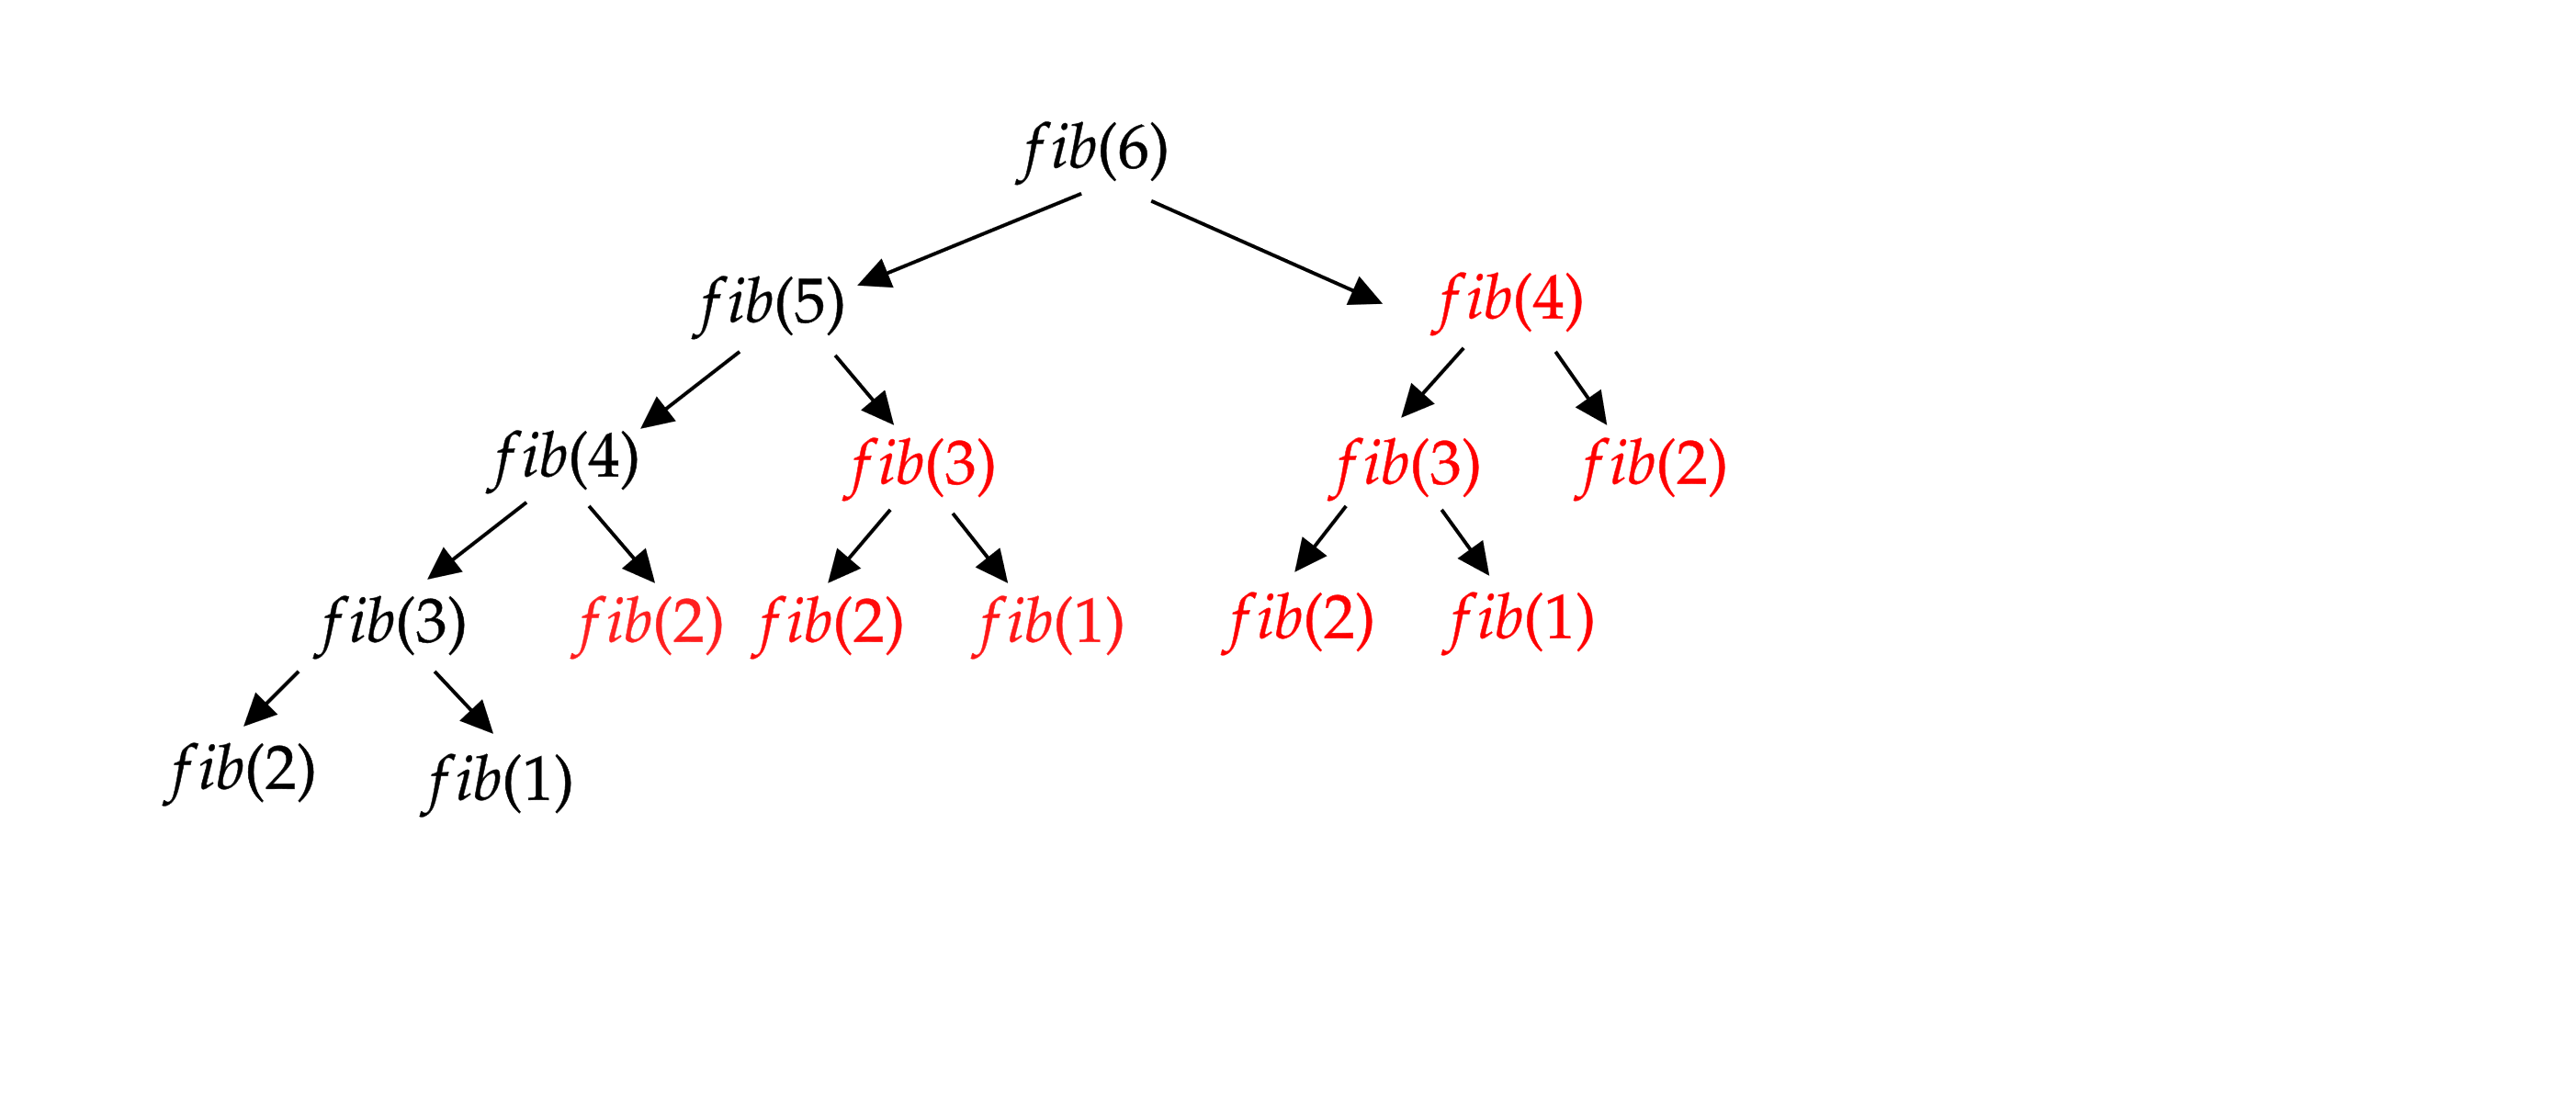
\includegraphics[width=1\textwidth]{Sections/dp/fib.png}

\vspace{-3em}
\caption{Recursion Tree for Fibonacci Sequence}
\label{fig:fib}
\end{figure}

\noindent
We see that we've already computed $F_2$ and $F_3$ multiple times. We can store these values in a table, and use them when needed:

\begin{Func}[Memo Fibonacci Sequence - \textit{Fib()}]

    \textbf{Input:} $n$ the index of the Fibonacci sequence we wish to compute.\\
    \textbf{Output:} $F_n$ the $n_{th}$ Fibonacci number.\\

    \vspace{-.5em}
    \begin{algorithm}[H]
        \SetAlgoLined
        \SetKwProg{Fn}{Function}{:}{\KwRet{}}
        $F[\ ]$; \tcp{Table to store Fibonacci numbers}
        \Fn{\textit{Fib}($n$)}{
            \If{$n \leq 1$}{
                \textbf{return} $n$\;
            }
            \Else{
                \If{$F[n]$ is not defined}{
                    $F[n] = \textit{Fib}(n-1)+\textit{Fib}(n-2)$\;
                }
                \textbf{return} $F[n]$\;
            }
        }
    \end{algorithm}
    \rule{\textwidth}{0.4pt}
    \textbf{Time Complexity:} $O(n)$. Since we only need to compute $F_n$ once, we at most recurse $n-1$ times. As 
    we unravel we have all our necessary values stored in our table.\\
    \textbf{Space Complexity:} $O(n)$. We store $n$ and recurse at most $n-1$ times.
\end{Func}


\newpage
\noindent
\textbf{Scenario - \textit{Weighted Interval Scheduling}}: Say we have $n$ paying jobs which overlap each other.
We want to find the best set of jobs that allows us to maximize our profit. Recall Section (\ref{sec:interval})

\begin{figure}[h]
\centering
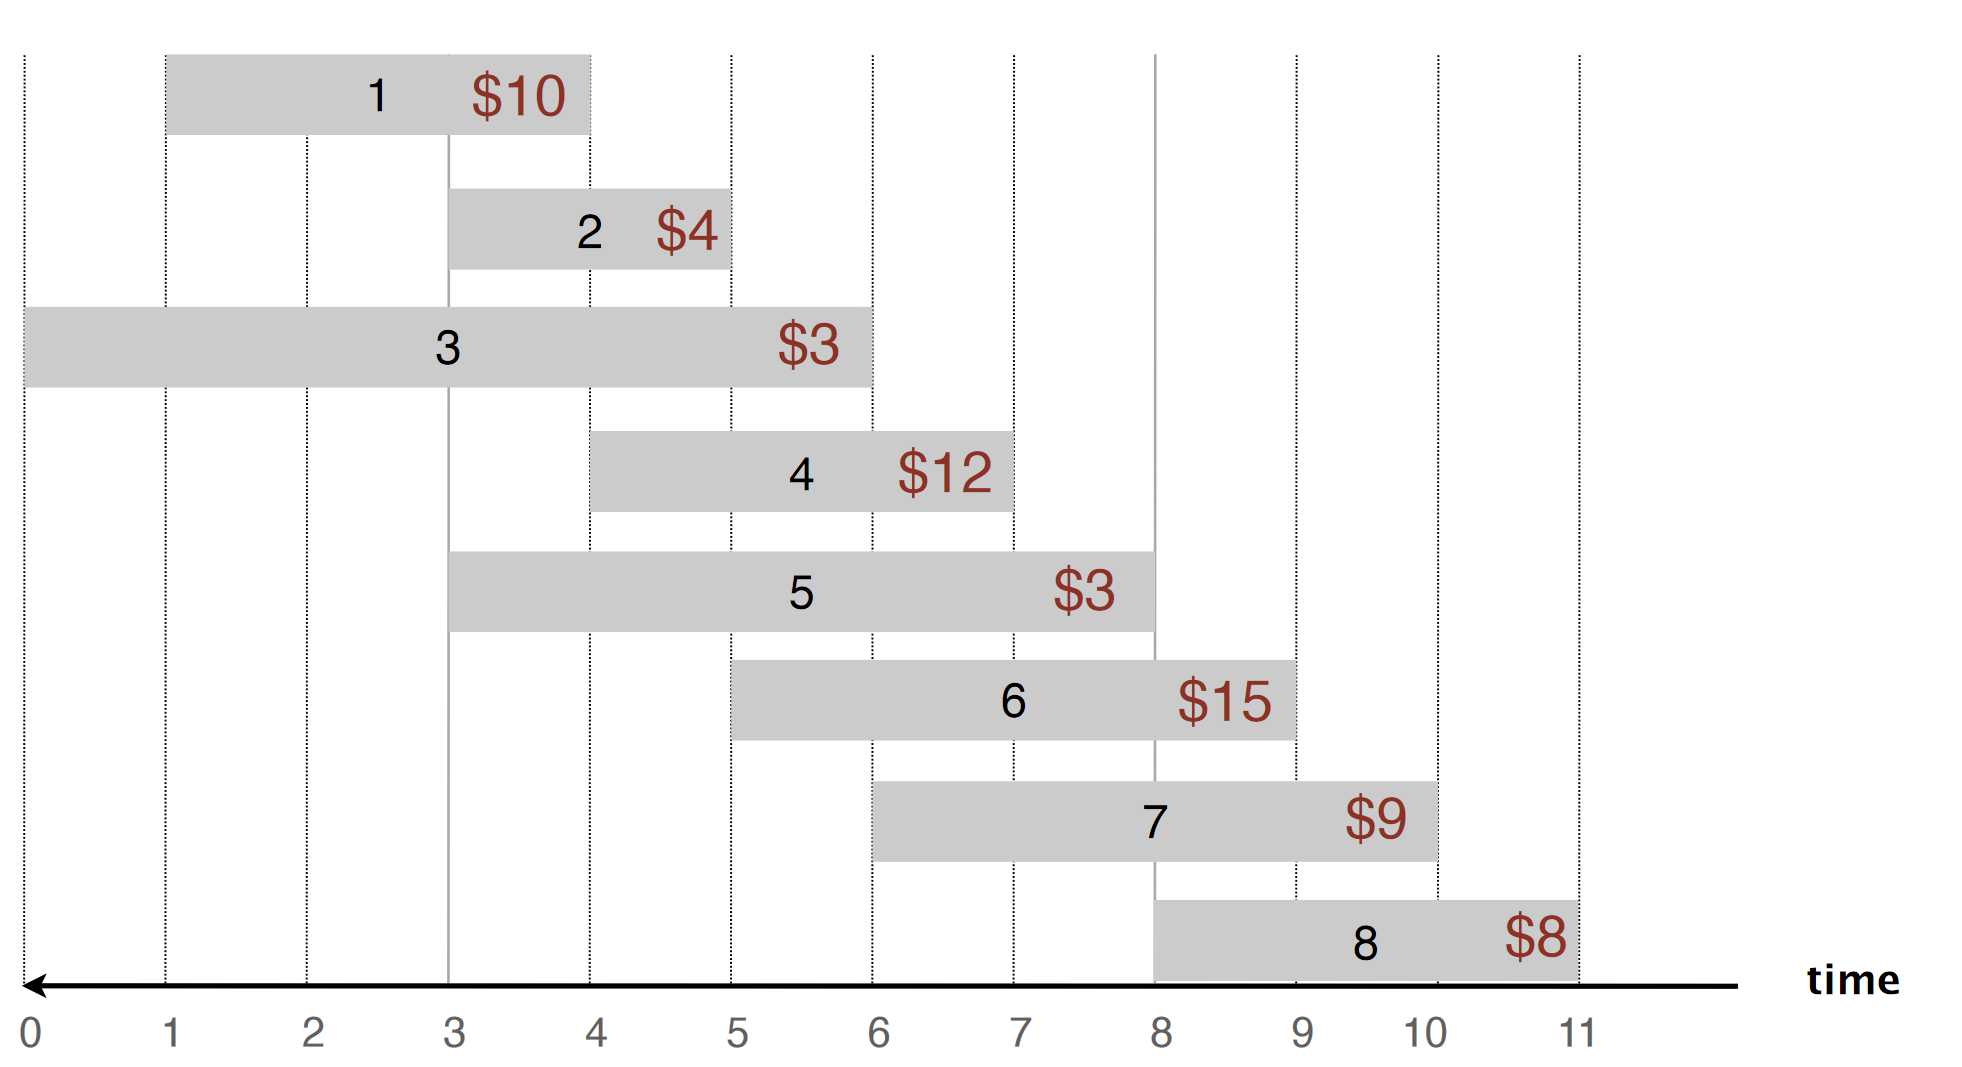
\includegraphics[width=.7\textwidth]{Sections/dp/wis.png}
\end{figure}

\noindent
Let us define $\mathbf{OPT(j)}$ as the maximum profit from jobs $\{1\dots j\}$, and $\mathbf{v_j}$ as $j_{th}$'s value. Then $OTP(8)$, considers jobs $1\dots 8$. Let $p(j):=$ The largest index $i < j$, s.t., job $i$ is compatible with $j$.\\
(if none, then $p(j) = 0$). We have two cases: 

\vspace{-1em}
\begin{align*}
    OPT(8) =
    \begin{cases}
        OPT(7) & \text{if job 8 is not selected}\\
        v_8 + OPT(p(8)) & \text{if job 8 is selected}
    \end{cases}
\end{align*}

\noindent
As $p(8)=5$, $p(5)$ is undefined, yielding $\$11$, which isn't the optimal solution, see job 6.

\noindent
If we don't choose $j$, then the optimal solution resides in $\{1\dots j-1\}$. So we want to know, 
if our current $OPT()$ solution larger than the next solution. We derive the following cases, and algorithm:
\begin{align*}
    OPT(j) =
    \begin{cases}
        0 & \text{if $j=0$}\\
        max\{v_j+OPT(p(j)), OPT(j-1)\} & \text{else}
    \end{cases}
\end{align*}

\vspace{-1em}
\begin{Func}[Weighted Interval Scheduling - \textit{OPT()}]
    
    \vspace{-.5em}
    Compute all $OPT(j)$ recursivley, unraveling seeing which $OPT(j)$ is larger; $\mathbf{O(2^n)}$ \textbf{Time}.\\
        \begin{algorithm}[H]
            \SetAlgoLined
            \SetKwProg{Fn}{Function}{:}{}
            \Fn{\textit{OPT}($j$)}{
                \If{$j = 0$}{
                    \textbf{return} $0$\;
                }
                \Else{
                    $OPT(j) \gets max\{v_j+OPT(p(j)), OPT(j-1)\}$\;
                    \textbf{return} $OPT(j)$\;
                }
            }
        \end{algorithm}
    \end{Func}

    \newpage

    \noindent
    Now we employ memoization to store our results in a table, and use them when needed:

    \begin{Func}[Memo Weighted Interval Scheduling - \textit{OPT()}]
        
        \vspace{-.5em}
        \begin{algorithm}[H]
            Sort jobs by finish time; \tcp{$O(n\log n)$}
            Compute all $p(1),\dots,p(n)$; \tcp{$O(n)$}
            \SetKwProg{Fn}{Function}{:}{}
            $OPT[\ ]$; \tcp{Table to store $OPT(j)$}
            \Fn{\textit{OPT}($j$)}{
                \If{$j = 0$}{
                    \textbf{return} $0$\;
                }
                \Else{
                    \If{$OPT[j]$ is not defined}{
                        $OPT[j] \gets max\{v_j+OPT(p(j)), OPT(j-1)\}$; \tcp{$O(n)$}
                    }
                    \textbf{return} $OPT[j]$\;
                }
            }
        \end{algorithm}
        \rule{\textwidth}{0.4pt}
        \textbf{Time Complexity:} $O(n\log n)$, as we are bottle-necked by our sorting algorithm. Line 10 is $O(n)$, following 
        the same memoization pattern as the Fibonacci sequence.
    \end{Func}

    \vspace{-2em}
    \section{Bottom-Up Dynamic Programming}
    In the fibonacci, sequence we don't have to compute it recursively. As shown before we can compute it linearly. Computing $F_5$, we do $0+1=1$, $1+1=2$, $1+2=3$, and $2+3=5$.
    
    \begin{Func}[Bottom-Up Fibonacci Sequence - \textit{Fib()}]
        
        \vspace{-.5em}
        \begin{algorithm}[H]
            \SetAlgoLined
            \SetKwProg{Fn}{Function}{:}{}
            $F[0] \gets 0$; $F[1] \gets 1$; \tcp{Base cases (array of size $n+1$)}
            \For{$i \gets 2$ \KwTo $n$}{
                $F[i] \gets F[i-1]+F[i-2]$\;
            }
            \textbf{return} $F[n]$\;
        \end{algorithm}
        \rule{\textwidth}{0.4pt}
        \textbf{Time Complexity:} $O(n)$. We compute $F_n$ linearly, only needing to compute $F_i$ once.
    \end{Func}
    \noindent
    To offer intuition, recall figure (\ref{fig:fib}), we see that that we only really take one branch of the tree. All other branches are 
    redundant. I.e., it's almost as if we have a linear path from the root to the leaf. Hence, there's no need for recursion.

    \newpage
    \noindent
    Likewise, we can compute the weighted interval scheduling problem linearly:
    \begin{Func}[Bottom-Up Weighted Interval Scheduling - \textit{OPT()}]
        
        \vspace{-.5em}
        \begin{algorithm}[H]
            \SetAlgoLined
            \SetKwProg{Fn}{Function}{:}{}
            Sort jobs by finish time; \tcp{$O(n\log n)$}
            Compute all $p(1),\dots,p(n)$; \tcp{$O(n)$}
            $OPT[0] \gets 0$; \tcp{Base case (array of size $n+1$)}
            \For{$j \gets 1$ \KwTo $n$}{
                $OPT[j] \gets max\{v_j+OPT(p(j)), OPT[j-1]\}$\;
            }
            \textbf{return} $OPT[n]$\;
        \end{algorithm}
        \rule{\textwidth}{0.4pt}
        \textbf{Time Complexity:} $O(n\log n)$. We sort our jobs, and compute $p(1),\dots,p(n)$ in $O(n)$ time. We then compute $OPT(j)$ linearly, only needing to compute $OPT(j)$ once.
    \end{Func}
    



